\documentclass[]{article}
\usepackage{lmodern}
\usepackage{amssymb,amsmath}
\usepackage{ifxetex,ifluatex}
\usepackage{fixltx2e} % provides \textsubscript
\ifnum 0\ifxetex 1\fi\ifluatex 1\fi=0 % if pdftex
  \usepackage[T1]{fontenc}
  \usepackage[utf8]{inputenc}
\else % if luatex or xelatex
  \ifxetex
    \usepackage{mathspec}
  \else
    \usepackage{fontspec}
  \fi
  \defaultfontfeatures{Ligatures=TeX,Scale=MatchLowercase}
\fi
% use upquote if available, for straight quotes in verbatim environments
\IfFileExists{upquote.sty}{\usepackage{upquote}}{}
% use microtype if available
\IfFileExists{microtype.sty}{%
\usepackage{microtype}
\UseMicrotypeSet[protrusion]{basicmath} % disable protrusion for tt fonts
}{}
\usepackage[margin=1in]{geometry}
\usepackage{hyperref}
\hypersetup{unicode=true,
            pdfborder={0 0 0},
            breaklinks=true}
\urlstyle{same}  % don't use monospace font for urls
\usepackage{longtable,booktabs}
\usepackage{graphicx,grffile}
\makeatletter
\def\maxwidth{\ifdim\Gin@nat@width>\linewidth\linewidth\else\Gin@nat@width\fi}
\def\maxheight{\ifdim\Gin@nat@height>\textheight\textheight\else\Gin@nat@height\fi}
\makeatother
% Scale images if necessary, so that they will not overflow the page
% margins by default, and it is still possible to overwrite the defaults
% using explicit options in \includegraphics[width, height, ...]{}
\setkeys{Gin}{width=\maxwidth,height=\maxheight,keepaspectratio}
\IfFileExists{parskip.sty}{%
\usepackage{parskip}
}{% else
\setlength{\parindent}{0pt}
\setlength{\parskip}{6pt plus 2pt minus 1pt}
}
\setlength{\emergencystretch}{3em}  % prevent overfull lines
\providecommand{\tightlist}{%
  \setlength{\itemsep}{0pt}\setlength{\parskip}{0pt}}
\setcounter{secnumdepth}{0}
% Redefines (sub)paragraphs to behave more like sections
\ifx\paragraph\undefined\else
\let\oldparagraph\paragraph
\renewcommand{\paragraph}[1]{\oldparagraph{#1}\mbox{}}
\fi
\ifx\subparagraph\undefined\else
\let\oldsubparagraph\subparagraph
\renewcommand{\subparagraph}[1]{\oldsubparagraph{#1}\mbox{}}
\fi

%%% Use protect on footnotes to avoid problems with footnotes in titles
\let\rmarkdownfootnote\footnote%
\def\footnote{\protect\rmarkdownfootnote}

%%% Change title format to be more compact
\usepackage{titling}

% Create subtitle command for use in maketitle
\newcommand{\subtitle}[1]{
  \posttitle{
    \begin{center}\large#1\end{center}
    }
}

\setlength{\droptitle}{-2em}

  \title{}
    \pretitle{\vspace{\droptitle}}
  \posttitle{}
    \author{}
    \preauthor{}\postauthor{}
    \date{}
    \predate{}\postdate{}
  

\begin{document}

\subsection{Excitation-emission
profiles}\label{excitation-emission-profiles}

\begin{center}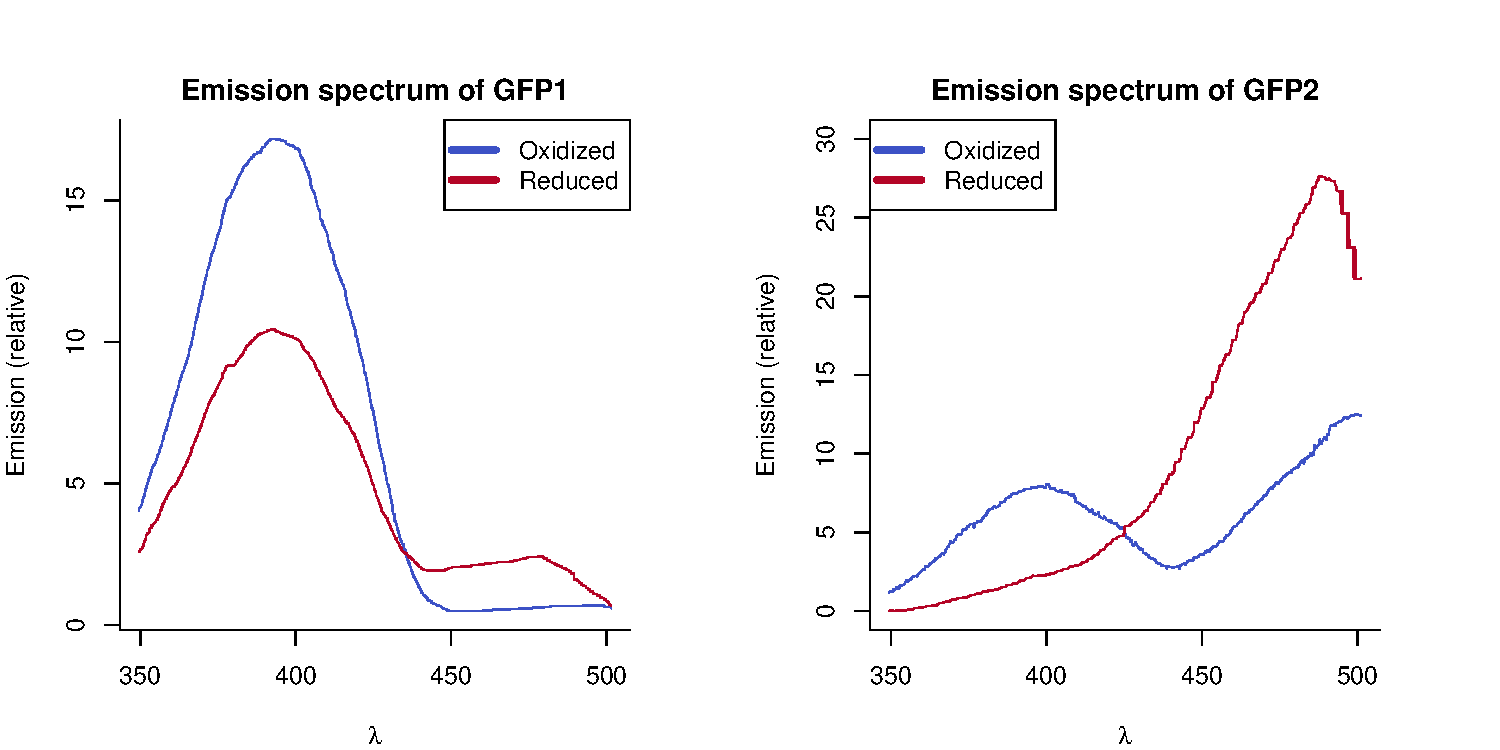
\includegraphics{Comparison_roGFP1_roGFP2_files/figure-latex/Plot spectra-1} \end{center}

\subsection{Delta profiles}\label{delta-profiles}

\begin{center}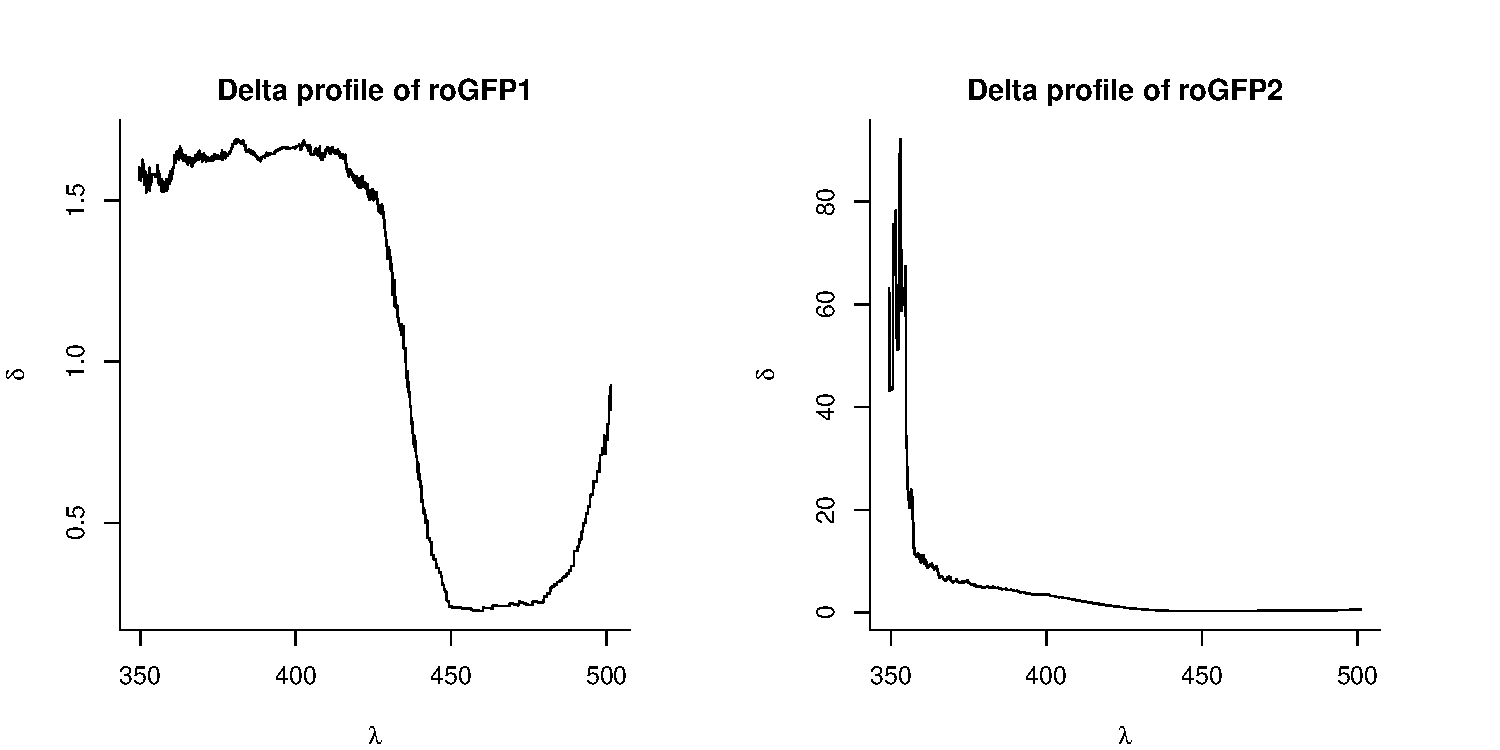
\includegraphics{Comparison_roGFP1_roGFP2_files/figure-latex/Plot deltas-1} \end{center}

\begin{longtable}[]{@{}lrr@{}}
\caption{Table 1: Approximate delta-wavelength values for GFP1 and GFP2
sensors}\tabularnewline
\toprule
Characteristic & GFP1 & GFP2\tabularnewline
\midrule
\endfirsthead
\toprule
Characteristic & GFP1 & GFP2\tabularnewline
\midrule
\endhead
Delta \textasciitilde{} 1 & 435.768 & 425.0872\tabularnewline
Delta minimized & 459.068 & 450.6872\tabularnewline
Delta maximized & 380.768 & 353.0872\tabularnewline
\bottomrule
\end{longtable}

Choose two sets of wavelengths for each sensor.

For GFP1:

\begin{itemize}
\tightlist
\item
  Use \(\frac{380 +/- 5 nm}{435 +/- 5 nm}\) for isobestic
\item
  Use \(\frac{380 +/- 5 nm}{460 +/- 5 nm}\) for maximum total dynamic
  range
\end{itemize}

For GFP2:

\begin{itemize}
\tightlist
\item
  Use \(\frac{360 +/- 5 nm}{425 +/- 5 nm}\) for isobestic
\item
  Use \(\frac{360 +/- 5 nm}{450 +/- 5 nm}\) for maximum total dynamic
  range
\end{itemize}

\begin{longtable}[]{@{}lrrrr@{}}
\caption{Table 2: Characteristics of GFP1 and GFP2
sensors}\tabularnewline
\toprule
Characteristic & GFP1 Isobestic & GFP1 Max & GFP2 Isobestic & GFP2
Max\tabularnewline
\midrule
\endfirsthead
\toprule
Characteristic & GFP1 Isobestic & GFP1 Max & GFP2 Isobestic & GFP2
Max\tabularnewline
\midrule
\endhead
Delta & 1.1 & 0.2 & 1.00 & 0.30\tabularnewline
Rmin & 3.3 & 4.3 & 0.05 & 0.02\tabularnewline
Rmax & 4.9 & 30.6 & 0.50 & 0.70\tabularnewline
E0 & -288.0 & -288.0 & -272.00 & -272.00\tabularnewline
Adjusted E0 & -289.5 & -269.6 & -271.50 & -256.00\tabularnewline
Dynamic Range & 1.6 & 26.3 & 0.50 & 0.70\tabularnewline
Fold Change & 1.5 & 7.1 & 11.50 & 38.80\tabularnewline
\bottomrule
\end{longtable}

\begin{center}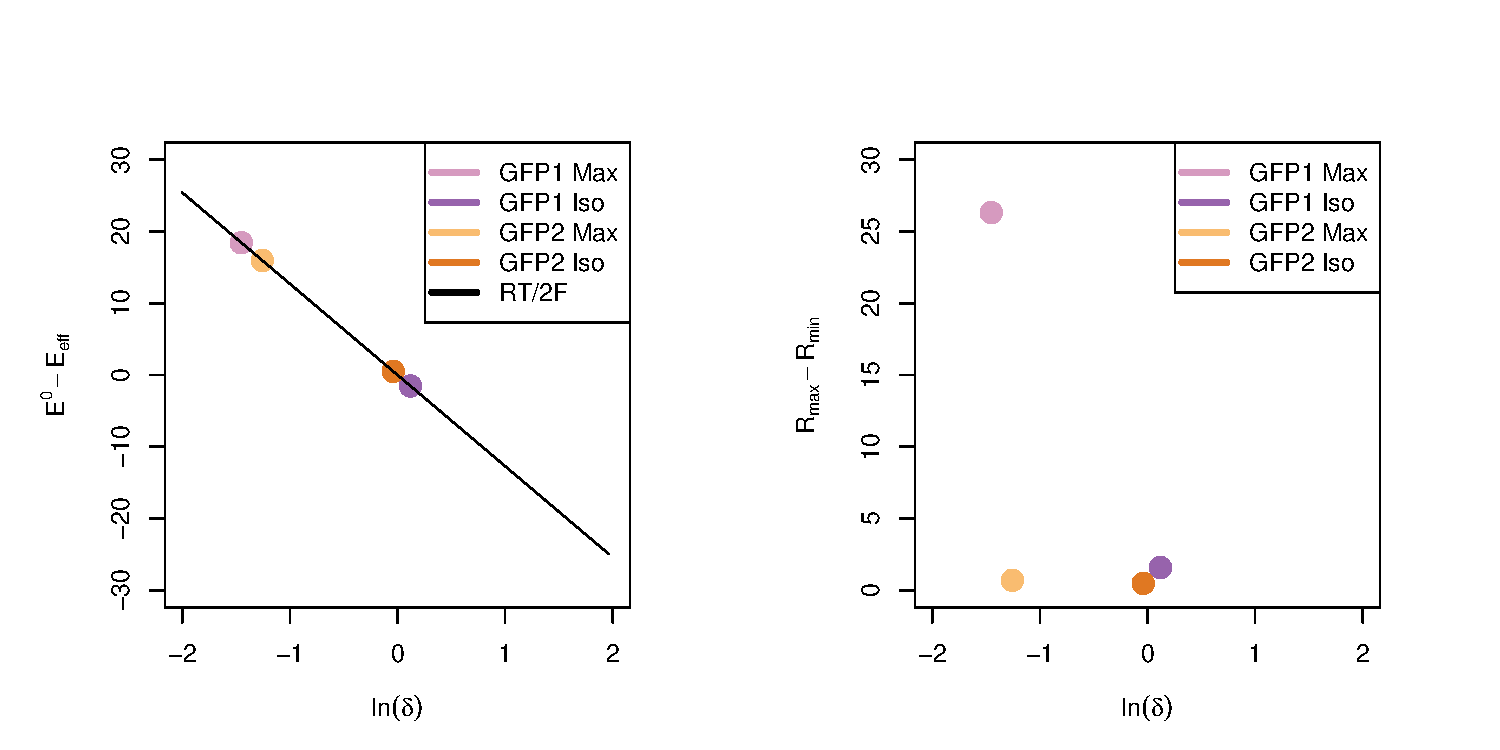
\includegraphics{Comparison_roGFP1_roGFP2_files/figure-latex/Characterize E0 and delta-1} \end{center}

\subsection{Fraction oxidized and redox
potential}\label{fraction-oxidized-and-redox-potential}

\begin{center}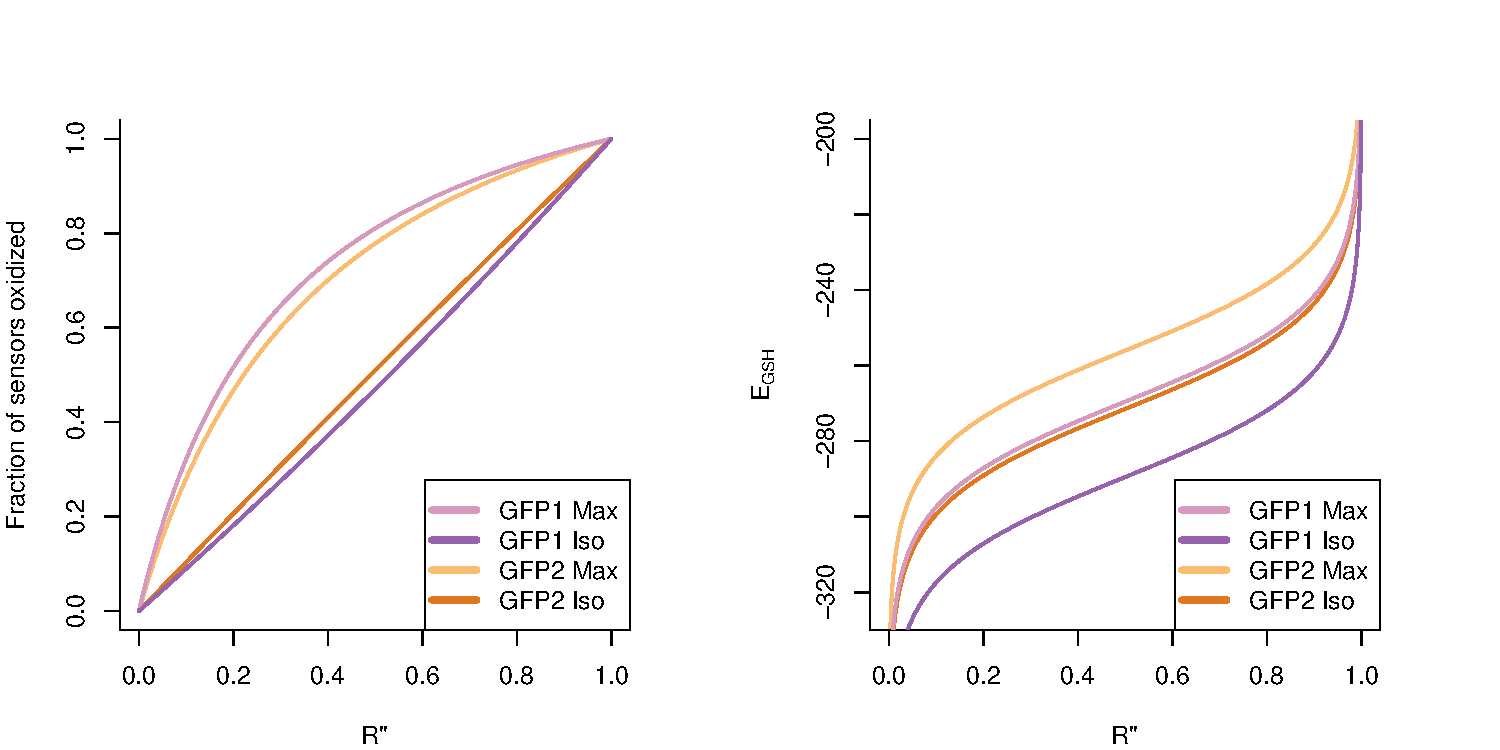
\includegraphics{Comparison_roGFP1_roGFP2_files/figure-latex/OxD and E-1} \end{center}

\begin{center}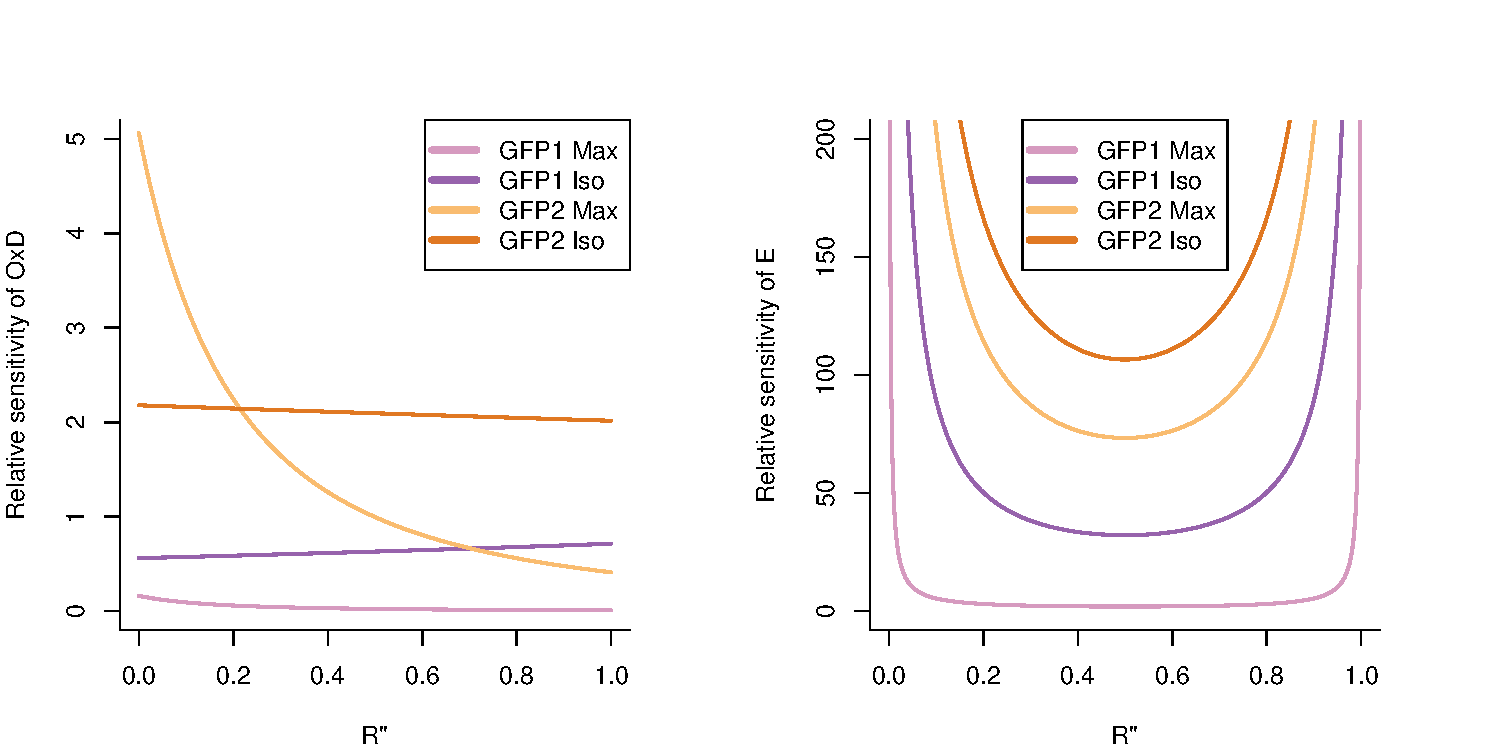
\includegraphics{Comparison_roGFP1_roGFP2_files/figure-latex/Sensitivity of E and OxD-1} \end{center}

\subsection{Sensitivity given 5\% error in
R}\label{sensitivity-given-5-error-in-r}

\begin{center}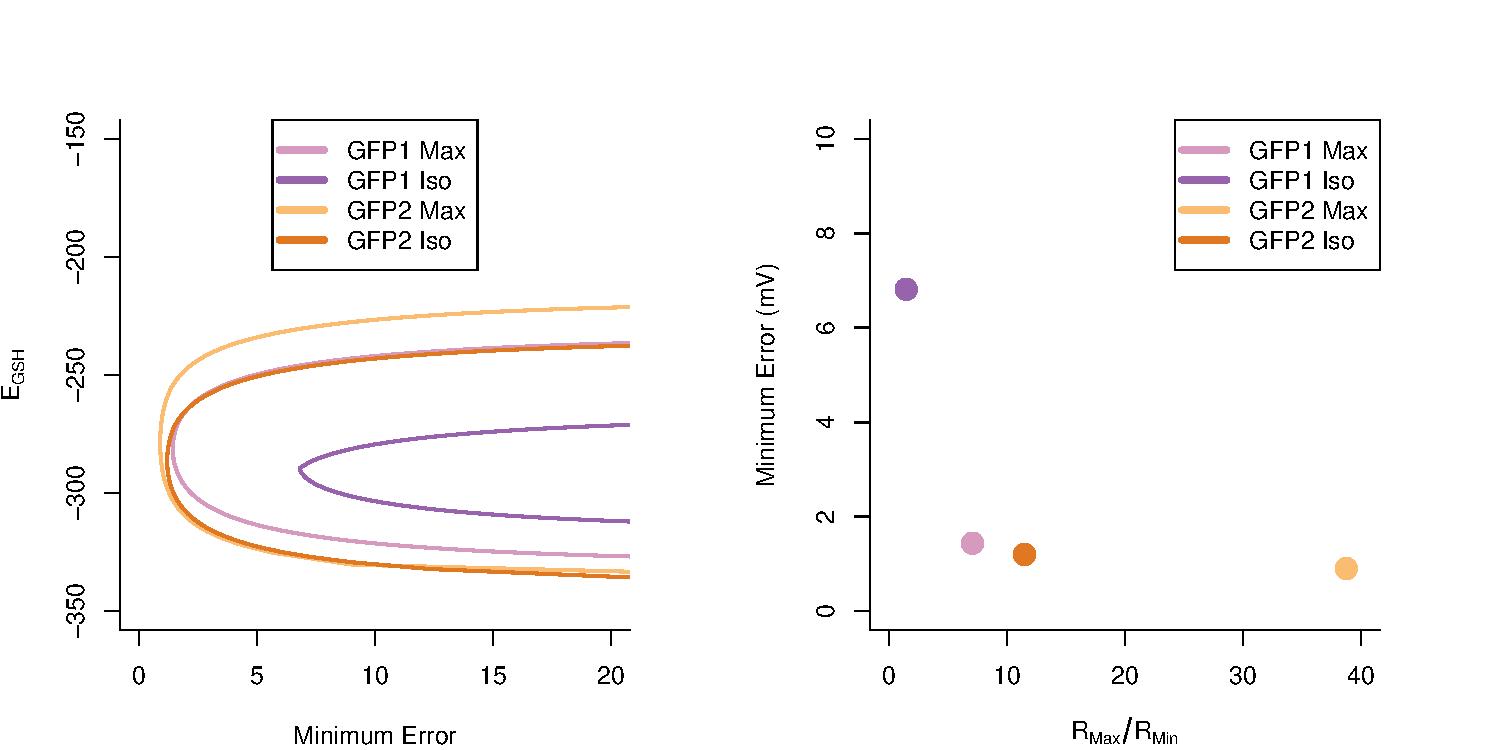
\includegraphics{Comparison_roGFP1_roGFP2_files/figure-latex/unnamed-chunk-1-1} \end{center}


\end{document}
